% Budget/contract: 1.1 pages. Main contribution section. Define task, label
% construction with no-trade band, chronological day-block splits with zero
% train/eval target-window overlap (no purge/embargo gap),
% dummy floors, readout metrics, predeclared criteria, validation-budget ledger,
% and Fig 1. Values from claims ledger v1.13: horizon_k=9 bars, band=3.0 bps;
% train 1998-01-02 -> 2013-09-16, validation -> 2017-01-25 (end exclusive).
\section{Task and Evaluation Protocol}\label{sec:protocol}

The protocol fixes the label, the splits, the baselines, the readout metric, and
the decision rules before the first model is scored. The decision margins we later report
are therefore prespecified, never a post hoc selection. Split-boundary controls
decide which rows are eligible to score, and a validation-budget ledger records
each logged contact with the validation split
\cite{kapoor2023leakage,lopezdeprado2018advances}. One limit is built in: we
exercise the protocol on a single near-null case with no known-signal positive
control. Its power to separate signal from noise rests on construction here,
not on a demonstration.

\subsection{Task}

The task is drop-neutral binary intraday direction classification on 5-minute
bars, resampled from 1-minute data for five US large-cap equities (CSCO, JPM,
KO, MSFT, WMT). One prediction unit is a single ticker at a single completed
5-minute target bar, scored up or down over a fixed forward horizon. Any edge
the protocol preserves is classification evidence, not economic value.

\subsection{Label}

Each row's label is the sign of the 9-bar-ahead forward return outside a no-trade
band. Writing \(\theta\) for the band in return units, a row is labeled up when
the forward return exceeds \(+\theta\) and down when it falls below \(-\theta\).
Any row inside the band is invalid and is dropped. We set \(\theta\) to \(3.0\) bps.
The band removes near-flat moves whose direction is set by noise
\cite{xu2018stock,sun2017predicting} and shifts the label distribution away from
the all-bars distribution \cite{zadrozny2004learning}. It also defines the
per-day activity proxy used by a later conditional diagnostic; that diagnostic is a
limitation rather than a result. Labels and windows are day-local and
per-ticker: no window and no label crosses a trading-day boundary or a ticker.
The surviving up and down rows are the only supervised rows, and no-trade rows
are neither a third class nor imputed.

\subsection{Chronological splits}

Chronological day blocks define the partitions and are fixed by the Stage~00
freeze \cite{hyndman2021forecasting}. Train runs from 1998-01-02 to 2013-09-16
(end exclusive), official validation from 2013-09-16 to 2017-01-25 (end
exclusive), and the holdout is closed from 2017-01-25 onward. No stage in the
validation pipeline reads or scores a post-2017 bar, and the run manifest records
holdout contact as false. The guarded walk-forward in
Section~\ref{sec:guarded} opens that segment only after the model is frozen, so
it confirms the frozen primary rather than testing it cleanly. Because every
window and horizon stays inside one trading day, the last train target window and
the first validation target window cannot straddle the cut or share a row. Within-day
locality substitutes for purge and embargo here; we apply neither. Cross-day serial
dependence therefore stays intact, which is a limitation, not a solved problem. Preprocessing that learns statistics is fit on
train rows alone and applied unchanged to validation. The feature window
\(w = 20\) is likewise set by a train-inner feature-and-window search
(Section~\ref{sec:setup}), not tuned on the validation readout.

\subsection{Baselines}

Every model score is read against same-row trivial baselines on the identical
target rows, within each evidence domain. The validation criteria use a
stratified dummy that samples from the empirical train label prior and a majority
baseline that always predicts the most frequent train label. The stratified dummy
pins a same-row, label-prior \macrofone{} floor for the drop-neutral target.
Reading every model on the identical rows against this prior closes the
class-imbalance illusion: a margin over it means ``above train-prior guessing,''
not a score inflated by base rates. That margin alone does not exclude serial structure or microstructure effects,
which later guards and diagnostics address.

\subsection{Readout metric and predeclared criteria}

We score the model-versus-dummy margin in \macrofone{} on the drop-neutral
up/down target. A dated protocol fixed the decision criteria before any readout
\cite{hofman2023preregistration}, and they apply to the predeclared TCN primary.
On the validation split the primary passes when its \macrofone{} delta is positive
over both the stratified dummy and the majority baseline. At least three of the
five tickers must also be positive, where three is a floor, not the achieved
count. These floors are deliberately weak: predeclaration
fixes the bar in advance, but it does not make the bar discriminating. The
guarded walk-forward carries its own separate and also weak predeclared stability
bar. Neither readout selects a model, and no final model is selected.

\subsection{Validation-budget ledger}

A validation-budget ledger counts and tier-tags every readout contact with the
official validation split, each carrying \texttt{for\_selection} set to false. It
makes those contacts traceable and bounds disclosed reuse; it is an internal count,
not an external timestamp. It later records \numseeds{} official-validation seed-candidate scoring
events against 56 guarded scoring events. The protocol keeps three evidence
domains separate and reports each number only within its own domain. These are the official
validation readout over \numseeds{} seeds, the train-inner control comparisons, and the guarded
non-independent walk-forward readout, also scored under the two prespecified seeds.
No reported number crosses domains.

Figure~\ref{fig:protocol-timeline} summarizes the timeline and the freeze ordering.

\begin{figure}[t]
  \centering
  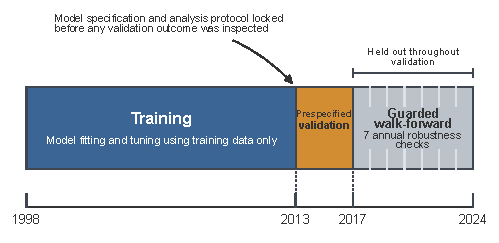
\includegraphics[width=\linewidth]{figures/fig_protocol_timeline}
  \Description{A single-row, to-scale timeline from 1998 to 2024 with three
    contiguous eras: a wide blue Training band labelled model fitting and
    tuning using training data only, a narrow amber Prespecified validation
    band, and a neutral-grey Guarded walk-forward era holding seven robustness
    checks, the final block longer than the 12-month width of the others. The
    phase and action labels are written inside the
    colored bands, while the lower axis carries only the boundary years 1998,
    2013, 2017, and 2024, with guide lines linking the 2013 and 2017 split
    boundaries to the colored bands. An arrow states that the model
    specification and analysis protocol were locked before any validation
    outcome was inspected. A bracket over the post-2017 era states that it was
    held out throughout validation. The caption states the freeze ordering,
    validation use, and non-independence limitation; split sizes and
    frozen-decision details are reported in the surrounding protocol and dataset
    table.}
  \caption{Protocol timeline and freeze ordering: training, one prespecified
    validation readout, then a guarded, non-independent post-2017 walk-forward.}
  \label{fig:protocol-timeline}
\end{figure}
